\documentclass{beamer}
\usepackage{wrapfig}
\usepackage{tikz}
\usepackage{tkz-berge} 
\usepackage{algorithm,algorithmic}
\mode<presentation>

{
  \usetheme{Warsaw}

 \setbeamertemplate{footline}{}
\setbeamercovered{transparent}
\usepackage{color}
\title{A programming approach to vertex coloring by kernelization}
\author{{Mehri Bagherihamaneh}\\[1cm]{\small {Advisor: Prof. Dr. Arie M.C.A. Koster}}\\[.5cm]{\small {Lehr-und Forschungsgebiet Diskrete Optimierung}}\\ {\small {Rheinisch-Westfaelische Technische Hochschule Aachen}}}

{\small \date{{Aachen, }\today}}


\begin{document}

\begin{frame}
  \titlepage
\end{frame}


\begin{frame}{What this thesis is about?}
\begin{itemize}

\item Graph vertex coloring

\item Using kernelization to solve vertex coloring with reduction of size of the  graph
\item Demonstrate kernelization in some sample graphs in practice
\item "improved DSATUR-based Branch and Bound" algorithm
\item Python is used as programming language

\end{itemize}
\end{frame}

\begin{frame}{Introduction}


\begin{enumerate}
\item Some definitions
\item Special kernelization for vertex coloring

\item Min vertex cover
\item An example

\item An exact algorithm for vertex coloring

\item Computational experiments
\item conclusion
\end{enumerate}
\end{frame}



\begin{frame}{Definitions}


\begin{definition}
A vertex coloring is an assignment of labels or colors to each
vertex of a graph such that no edge connects two vertices with the same color.

The chromatic number of a graph is the smallest number of colors needed for
vertex coloring and denoted by $\chi(G)$. 

A vertex coloring of a graph with $k$ or fewer colors is known as a $k$-coloring. A proper $k$-coloring is an assignment of $k$ colors to the vertices of a graph so that no two adjacent vertices have the same color. 

A proper $k$-coloring of a graph $G$ can be shown as a function $f: V(G) \to \{1, 2, 3, . . . , k\}$ such that adjacent vertices get different colors, namely in a proper coloring, for all edges $\{u, v\}$ we have $f(u) \not= f(v)$.
\end{definition}
\end{frame}


\begin{frame}{Definitions}
\begin{example}
The petersen graph is $3$-colorable:

\begin{center}
\begin{tikzpicture}[rotate=90]
  \GraphInit[vstyle=Hasse]
  \SetVertexNoLabel \SetUpVertex[MinSize=2pt] \grPetersen[RA=2,RB=1]
  \SetUpVertex[inner sep=1pt,MinSize=2pt]
  \AddVertexColor{red}{a0,b1,b2,a3}
  \AddVertexColor{green}{a1,b0,a4}
  \AddVertexColor{blue}{b4,b3,a2}
\end{tikzpicture}
\end{center}
\end{example}
\end{frame}

\begin{frame}{Propositional logic}
\begin{definition}
A propositional logic formula is constructed by some variables using operators AND ("$\land$"), OR ("$\lor$"), NOT ("$\lnot$") and parentheses. 

A clause is an expression constructed from a finite  disjunction or conjunction of literals.
\end{definition}



\begin{definition}
A boolean formula is satisfiable if it can be TRUE by assigning logical values to its variables. 
\end{definition}
\end{frame}
\begin{frame}{Propositional logic}


\begin{example}

\item $x_1 \land (x_2 \lor\lnot x_1)$, where $(x_2 \lor\lnot x_1)$ is a clause.

\end{example}
\begin{example}
 $\varphi = d\lor (a\land b\land (c\lor d \land\lnot a))$

\begin{table}[H]
\begin{center}
\begin{tabular}{c|c|c|c|c}
$a$ & $b$ & $c$ & $d$ & $\varphi$\\
\hline
F & F & F & T & T\\ 
&&&&\\
&&&&\\
\end{tabular}
\end{center}
\end{table}
\end{example}

\begin{example}
Unsatisfiable formula:

\begin{center}
$\theta = X \land \lnot X$
\end{center}
\end{example}

\end{frame}

\begin{frame}{Propositional logic}
\begin{definition}
A boolean formula is in conjunctive normal form (CNF) if it is a conjunction of one or more disjunctions of variables.
\end{definition}

\begin{example}
\item $\lnot x \land (y \lor z)$
\end{example}

\begin{definition}
For a given CNF formula $\varphi$, the boolean satisfiability problem (SAT) is a decision problem which asks whether the formula $\varphi$ is satisfiable. The $3$-SAT problem is a SAT problem with at most $3$ variables in each clause. 
\end{definition}

\begin{theorem}
The $3$-SAT problem is $NP$-complete.
\end{theorem}
\end{frame}


\begin{frame}{Complexity}
\begin{definition}
For an instance $I$ from instance set $\mathcal{I}$, a decision problem $\Pi$ is a YES-NO question which asks if
there is at least one solution for the problem $\Pi$ in $I$.
\end{definition}
\begin{example}
$k$-COLORING is a decision problem, which asks if we can color a graph $G$ with $k\in\mathbb{N}$ or fewer colors. For $k \geq 3$ in general graphs, $k$-COLORING is $NP$-complete.
\end{example}
\end{frame}


\begin{frame}{Complexity}
\begin{itemize}
\item class $P$ (PTIME)

\color{green} Example: \color{black} the problem of determining if a number is prime.

\item $NP$ (non-deterministic polynomial) $P\subset NP$.

\item $NP$-hard class 

\color{green} Example: \color{black} traveling salesman problem.

If $P \not= NP$, $NP$-hard problems cannot be solved in polynomial time. 

\item $NP$-complete class:  $L$ is $NP$-complete if:
\begin{enumerate}
\item $L$ is $NP$-hard.

\item $L$ is in $NP$.
\end{enumerate}
\end{itemize}
\end{frame}


\begin{frame}{Is $P = NP$ or $P \not= NP$?}

%\vspace{2cm}
\newcommand{\boundellipse}[3]% center, xdim, ydim
{(#1) ellipse (#2 and #3)
}

\begin{figure}[!ht]
\centering


\begin{tikzpicture}
\draw (0,0) circle (1.5cm);
\draw \boundellipse{0,-0.75}{1.1}{0.75};
\draw (-1.5,3) .. controls (-1,0) and (1,0) .. (1.5,3);
\node at (0,2) {\tiny $NP$-Hard};
\node at (0,1.2) {\tiny $NP$-Complete};
\node at (-1,0) {\tiny $NP$};
\node at (0,-0.75) {\tiny $P$};
\node at (0,-2) {\tiny $P \not= NP$};
\node at (4,1) [label={[rotate=90]{\tiny complexity}}];
\draw[->] (4,-2) -- (4,4);
\draw (8,0) circle (1.5cm);

\draw (6.5,2) .. controls (5.40,-2.7) and (10.6,-2.7) .. (9.5,2);
\node at (8,2) {\tiny $NP$-Hard};
\node at (8,0) {\tiny $NP$-Complete = $P$ = $NP$};

\node at (8,-2) {\tiny $P = NP$};
\end{tikzpicture}
\caption{\tiny Euler diagram for $P$, $NP$, $NP$-hard and $NP$-complete set of problems}
\end{figure}
\end{frame}

\begin{frame}{Parameterized Complexity}

If we assume $P \not = NP$, for small parameter  $k$ (but large instance), we can use efficient exact algorithms. 

\begin{definition}
A parameterized problem is a pair $(\Pi, \kappa)$ in which $\Pi$ is a
decision problem with instance set $\mathcal{I}$ and $\kappa : \mathcal{I} \to \mathbb{N}$, which is a polynomial
time computable function, called parameter.
\end{definition}

\begin{example}
Parameterized-vertex cover, denoted $k$-VERTEX COVER:

Input : graph $G = (V, E)$ and a number $k \in \mathbb{N}$

parameter : $k$

problem : Is there any vertex cover set in $G$ with maximum size of $k$?
\end{example}

\end{frame}

\begin{frame}{Kernelization}

\begin{definition}
Let $(\Pi, \kappa)$ be a parameterized problem, $I\in\mathcal{I}$ an instance and $\kappa: \mathcal{I} \to \mathbb{N}$ a parameterization for $\Pi$:

A polynomial time computable function $f : \mathcal{I} \times \mathbb{N} \to \mathcal{I} \times \mathbb{N}$ is called a
kernelization for $(\Pi, \kappa)$ , if $f(I, \kappa(I)) = (I', \kappa(I'))$ such that it satisfies these 3 properties:

\begin{enumerate}[(i)]
\item For each $I \in \mathcal{I}$, $(I, \kappa(I))$ is a "YES"-instance of $\Pi$ iff $(I', \kappa(I'))$ is a "YES"-instance of $\Pi$.

\item There is a function $f': \mathbb{N} \to \mathbb{N}$, such that $|I'| \leq f'(\kappa(I))$

\item $\kappa(I')\leq \kappa(I)$.
\end{enumerate}

$I'$ is kernel of $(\Pi, \kappa)$ and $f'(\kappa(I))$ is called the size of the kernel.

\end{definition}

\end{frame}

\begin{frame}{Kernelization}
\begin{example}
Kernelization of the vertex cover problem:

Input: Graph $G$ and a positive integer $k$ 

Output: A vertex cover set with at most size $k$


\begin{itemize}
\item If $v$ is an isolated vertex of $G$, we remove $v$. The new instance is $(G - v , k)$.


\item If $G$ contains a vertex $v$ of degree greater than $k$, remove $v$ from the graph and decrease $k$ by one. The new instance is $(G - v , k - 1)$.

\item If neither of the previous two rules can be applied anymore,
\begin{itemize}
\item If the graph still has more than $k^2$ edges, the problem has no solution.

\item If the graph has at most $k^2$ edges, it has at most $2 k^2$ vertices, hence the size of the kernel is at most $2 k^2$.
\end{itemize}

  
\end{itemize}



The problem can be solved in time $\mathcal{O}(2^{2k^2} + |V| + |E|)$.
\end{example}
\end{frame}


\begin{frame}{Kernelization of the Vertex Coloring}
A kernelization on $3$-coloring using vertex cover:

\begin{enumerate}
\item Compute $2$-approximate vertex cover $X$

\item $\forall S\subseteq X$ of size $3$
\begin{itemize}
\item Mark a common neighbor of $S$
\end{itemize}
\item Delete all unmarked $v \not\in X$

\item Output resulting $G'$ on $n'$ vertices:

\begin{center}
$n' \leq |X| + |X|^3 \leq 2k + (2k)^3$
\end{center}
\end{enumerate}

$G$ is $3$-colorable iff $G'$ is $3$-colorable. Run time for the algorithm is $\mathcal{O}(min|X|^3)$.


\begin{theorem}{\label{main theorem}}
$G$ is $q$-colorable iff $G'$ is $q$-colorable. Run time for the algorithm
is $\mathcal{O}(min|X|^q)$.
\end{theorem}
\end{frame}

\begin{frame}{Revision of the algorithm}

\begin{algorithm}[H]
\begin{algorithmic}[1]
\SetAlgoLined
\DontPrintSemicolon
  \caption{Kernelization of vertex coloring by using vertex cover}

\STATE Find exact minimum vertex cover\\

\STATE Iterate all vertices outside of vertex cover\\

\STATE If the vertex has $3$ distinct neighbors in vertex cover and it wasn't
visited yet, then mark it\\

\STATE Delete all unmarked vertices outside of vertex cover\\
\end{algorithmic}
\end{algorithm}
\end{frame}


\begin{frame}{Minimum Vertex Cover}

\begin{align*}
&minimize \; \;\; \; \sum_{v\in V}X_v \\
&subject\; to \;\;\; \; X_u + X_v  \geq 1 , \qquad \\
&\qquad 	\qquad\qquad\qquad	 \forall \{u,v\} \in E\\
&and	\qquad\qquad	 \forall v, X_v\in \{0,1\}
\end{align*}
\end{frame}


\begin{frame}{Minimum Vertex Cover}
We can restrict this ILP to maximal cliques inequality:


\begin{align*}
&minimize \; \;\; \; \sum_{v\in V}X_v\\
&subject\; to \;\;\; \; X_u + X_v  \geq 1 ,\\
&\qquad 	\qquad\qquad\qquad	 \forall \{u,v\} \in E\\
&and	\qquad\quad\;\; \sum_{v\in K_n}x_v \geq n - 1\\
& \qquad\qquad \qquad\qquad for\; every\; maximal\; clique\; K_n\; in\; the\; graph\\
&and	\qquad\qquad	 \forall v, X_v\in \{0,1\}
\end{align*}
\end{frame}


\begin{frame}{Minimum Vertex Cover}
Every edge is also a clique:


\begin{align*}
&minimize \; \;\; \; \sum_{v\in V}X_v\\
&subject\; to \;\;\; \; \sum_{v\in K_n}x_v \geq n - 1\\
& \qquad\qquad \qquad\qquad for\; every\; maximal\; clique\; K_n\; in\; the\; graph\\
&and	\qquad\qquad	 \forall v, X_v\in \{0,1\}
\end{align*}



\end{frame}

\begin{frame}{Maximal Clique}


\begin{algorithm}[H]
\begin{algorithmic}[1]

\STATE BronKerbosch({$R, P, X$})\\

        \IF{$P$ and $X$ are both empty}{
        
		  	 report $R$ as a maximal clique\\	
		 }\ENDIF
		\FOR{vertex $v$ in $P$}{
		
			   BronKerbosch$(R \cup \{v\}, P \cap N(v), X \cap N(v))$
			   
			    $P := P\setminus \{v\}$
			    
			   	   $X := X\cup \{v\}$\\
		}\ENDFOR

\end{algorithmic}
\caption{Bron-Kerbosch}
\end{algorithm}

\end{frame}

\begin{frame}{An Example}
This graph has $11$ vertices and $20$ edges and is known to be $4$-colorable:

\vspace{0.5cm}
\begin{center}
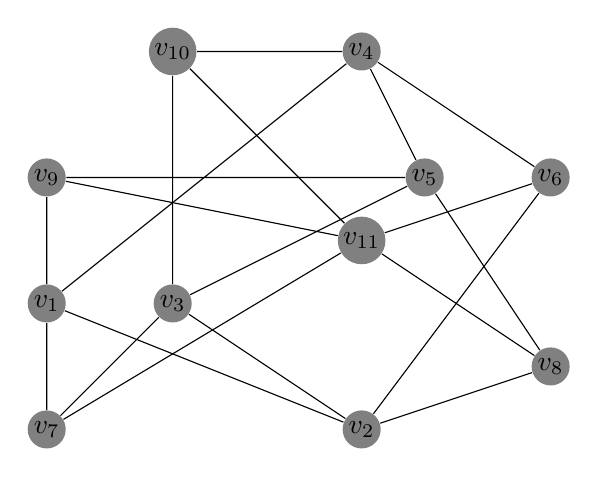
\begin{tikzpicture}[scale=0.8]
\node[circle,fill=gray,inner sep=1pt,minimum size=1mm] (v1) at (0,0) {$v_1$};
\node[circle,fill=gray,inner sep=1pt,minimum size=1mm] (v2) at (5,-2) {$v_2$};
\node[circle,fill=gray,inner sep=1pt,minimum size=1mm] (v3) at (2,0) {$v_3$};
\node[circle,fill=gray,inner sep=1pt,minimum size=1mm] (v4) at (5,4) {$v_4$};
\node[circle,fill=gray,inner sep=1pt,minimum size=1mm] (v5) at (6,2) {$v_5$};
\node[circle,fill=gray,inner sep=1pt,minimum size=1mm] (v6) at (8,2) {$v_6$};
\node[circle,fill=gray,inner sep=1pt,minimum size=1mm] (v7) at (0,-2) {$v_7$};
\node[circle,fill=gray,inner sep=1pt,minimum size=1mm] (v8) at (8,-1) {$v_8$};
\node[circle,fill=gray,inner sep=1pt,minimum size=1mm] (v9) at (0,2) {$v_9$};
\node[circle,fill=gray,inner sep=1pt,minimum size=1mm] (v10) at (2,4) {$v_{10}$};
\node[circle,fill=gray,inner sep=1pt,minimum size=1mm] (v11) at (5,1) {$v_{11}$};


\draw (v4)--(v1)--(v2)--(v3)--(v5)--(v9)--(v1);
\draw (v1)--(v7)--(v3)--(v10)--(v4)--(v6)--(v2)--(v8)--(v11);
\draw (v7)--(v11)--(v10);
\draw (v9)--(v11)--(v6);
\draw (v4)--(v5)--(v8);
\end{tikzpicture}
\end{center}


\end{frame}
\begin{frame}{Step 1}

Exact minimum vertex cover: $X = \{v_1 , v_2 , v_3 , v_4 , v_5 , v_{11}\}$ vs. $2$-approximate: $Y = \{v_1 , v_2 , v_3 , v_4 , v_5 , v_6 , v_8 , v_9 , v_{10} , v_{11}\}$.

\begin{center}
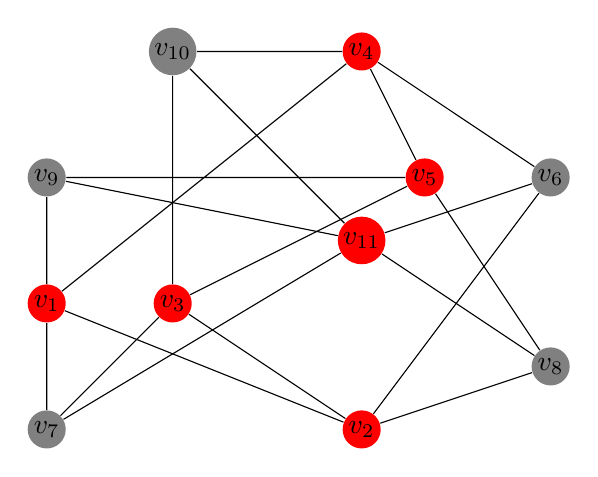
\begin{tikzpicture}[scale=0.8]
\node[circle,fill=red,inner sep=1pt,minimum size=1mm] (v1) at (0,0) {$v_1$};
\node[circle,fill=red,inner sep=1pt,minimum size=1mm] (v2) at (5,-2) {$v_2$};
\node[circle,fill=red,inner sep=1pt,minimum size=1mm] (v3) at (2,0) {$v_3$};
\node[circle,fill=red,inner sep=1pt,minimum size=1mm] (v4) at (5,4) {$v_4$};
\node[circle,fill=red,inner sep=1pt,minimum size=1mm] (v5) at (6,2) {$v_5$};
\node[circle,fill=gray,inner sep=1pt,minimum size=1mm] (v6) at (8,2) {$v_6$};
\node[circle,fill=gray,inner sep=1pt,minimum size=1mm] (v7) at (0,-2) {$v_7$};
\node[circle,fill=gray,inner sep=1pt,minimum size=1mm] (v8) at (8,-1) {$v_8$};
\node[circle,fill=gray,inner sep=1pt,minimum size=1mm] (v9) at (0,2) {$v_9$};
\node[circle,fill=gray,inner sep=1pt,minimum size=1mm] (v10) at (2,4) {$v_{10}$};
\node[circle,fill=red,inner sep=1pt,minimum size=1mm] (v11) at (5,1) {$v_{11}$};


\draw (v4)--(v1)--(v2)--(v3)--(v5)--(v9)--(v1);
\draw (v1)--(v7)--(v3)--(v10)--(v4)--(v6)--(v2)--(v8)--(v11);
\draw (v7)--(v11)--(v10);
\draw (v9)--(v11)--(v6);
\draw (v4)--(v5)--(v8);
\end{tikzpicture}
\end{center}

\end{frame}


\begin{frame}{Steps 2 and 3}
Outside vertices: $\{v_6, v_7, v_8, v_9, v_{10}\}$


For $q = 4$ and the vertex cover $X$, 
\begin{itemize}

\item $v_6$ has no $4$ neighbors in $X$.

\item $v_7$, $v_8$, $v_9$ and $v_{10}$ have no $4$ neighbors in $X$, either. 
\end{itemize}
\begin{center}
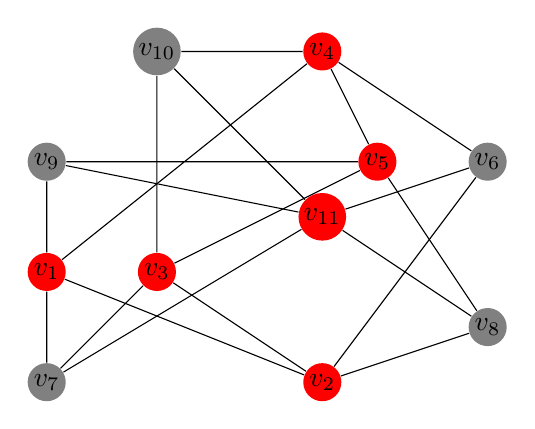
\begin{tikzpicture}[scale=0.7]
\node[circle,fill=red,inner sep=1pt,minimum size=1mm] (v1) at (0,0) {$v_1$};
\node[circle,fill=red,inner sep=1pt,minimum size=1mm] (v2) at (5,-2) {$v_2$};
\node[circle,fill=red,inner sep=1pt,minimum size=1mm] (v3) at (2,0) {$v_3$};
\node[circle,fill=red,inner sep=1pt,minimum size=1mm] (v4) at (5,4) {$v_4$};
\node[circle,fill=red,inner sep=1pt,minimum size=1mm] (v5) at (6,2) {$v_5$};
\node[circle,fill=gray,inner sep=1pt,minimum size=1mm] (v6) at (8,2) {$v_6$};
\node[circle,fill=gray,inner sep=1pt,minimum size=1mm] (v7) at (0,-2) {$v_7$};
\node[circle,fill=gray,inner sep=1pt,minimum size=1mm] (v8) at (8,-1) {$v_8$};
\node[circle,fill=gray,inner sep=1pt,minimum size=1mm] (v9) at (0,2) {$v_9$};
\node[circle,fill=gray,inner sep=1pt,minimum size=1mm] (v10) at (2,4) {$v_{10}$};
\node[circle,fill=red,inner sep=1pt,minimum size=1mm] (v11) at (5,1) {$v_{11}$};


\draw (v4)--(v1)--(v2)--(v3)--(v5)--(v9)--(v1);
\draw (v1)--(v7)--(v3)--(v10)--(v4)--(v6)--(v2)--(v8)--(v11);
\draw (v7)--(v11)--(v10);
\draw (v9)--(v11)--(v6);
\draw (v4)--(v5)--(v8);
\end{tikzpicture}
\end{center}
\end{frame}

\begin{frame}{Step 4}
All of the vertices out of $X$ are unmarked and will be removed. Then the output(kernel) is the set
$\{v_1 , v_2 , v_3 , v_4 , v_5 , v_{11}\}$:


\vspace{1cm}

\begin{center}
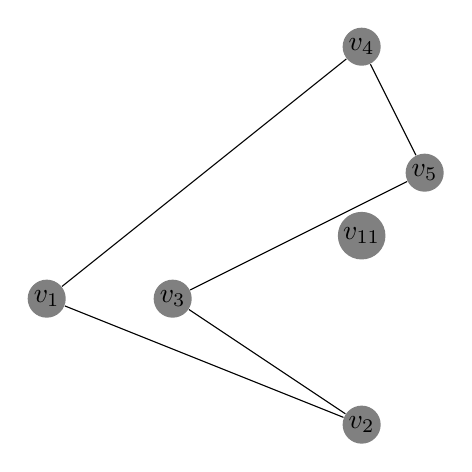
\begin{tikzpicture}[scale=0.8]
\node[circle,fill=gray,inner sep=1pt,minimum size=1mm] (v1) at (0,0) {$v_1$};
\node[circle,fill=gray,inner sep=1pt,minimum size=1mm] (v2) at (5,-2) {$v_2$};
\node[circle,fill=gray,inner sep=1pt,minimum size=1mm] (v3) at (2,0) {$v_3$};
\node[circle,fill=gray,inner sep=1pt,minimum size=1mm] (v4) at (5,4) {$v_4$};
\node[circle,fill=gray,inner sep=1pt,minimum size=1mm] (v5) at (6,2) {$v_5$};
\node[circle,fill=gray,inner sep=1pt,minimum size=1mm] (v11) at (5,1) {$v_{11}$};


\draw (v4)--(v1)--(v2)--(v3)--(v5);
\draw (v4)--(v5);
\end{tikzpicture}
\end{center}
\end{frame}

\begin{frame}{Coloring}

This kernel can be colored with $3$ and therefore with $4$ colors.

\begin{center}
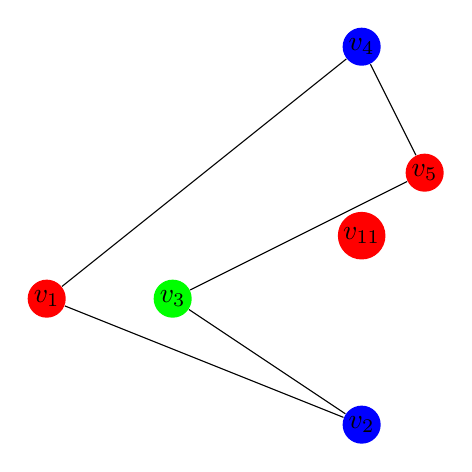
\begin{tikzpicture}[scale=0.8]
\node[circle,fill=red,inner sep=1pt,minimum size=1mm] (v1) at (0,0) {$v_1$};
\node[circle,fill=blue,inner sep=1pt,minimum size=1mm] (v2) at (5,-2) {$v_2$};
\node[circle,fill=green,inner sep=1pt,minimum size=1mm] (v3) at (2,0) {$v_3$};
\node[circle,fill=blue,inner sep=1pt,minimum size=1mm] (v4) at (5,4) {$v_4$};
\node[circle,fill=red,inner sep=1pt,minimum size=1mm] (v5) at (6,2) {$v_5$};
\node[circle,fill=red,inner sep=1pt,minimum size=1mm] (v11) at (5,1) {$v_{11}$};


\draw (v4)--(v1)--(v2)--(v3)--(v5);
\draw (v4)--(v5);
\end{tikzpicture}
\end{center}

\end{frame}
\begin{frame}{Another Steps 3 and 4}
For $q = 3$, and the vertex cover $X$, mark these vertices: $\{v_6, v_7, v_8, v_9, v_{10}\}$:
\begin{wrapfigure}{l}{4cm}
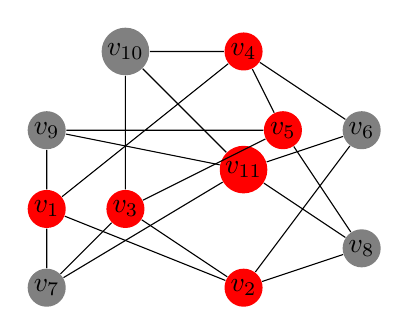
\begin{tikzpicture}[scale=0.5]
\node[circle,fill=red,inner sep=1pt,minimum size=1mm] (v1) at (0,0) {$v_1$};
\node[circle,fill=red,inner sep=1pt,minimum size=1mm] (v2) at (5,-2) {$v_2$};
\node[circle,fill=red,inner sep=1pt,minimum size=1mm] (v3) at (2,0) {$v_3$};
\node[circle,fill=red,inner sep=1pt,minimum size=1mm] (v4) at (5,4) {$v_4$};
\node[circle,fill=red,inner sep=1pt,minimum size=1mm] (v5) at (6,2) {$v_5$};
\node[circle,fill=gray,inner sep=1pt,minimum size=1mm] (v6) at (8,2) {$v_6$};
\node[circle,fill=gray,inner sep=1pt,minimum size=1mm] (v7) at (0,-2) {$v_7$};
\node[circle,fill=gray,inner sep=1pt,minimum size=1mm] (v8) at (8,-1) {$v_8$};
\node[circle,fill=gray,inner sep=1pt,minimum size=1mm] (v9) at (0,2) {$v_9$};
\node[circle,fill=gray,inner sep=1pt,minimum size=1mm] (v10) at (2,4) {$v_{10}$};
\node[circle,fill=red,inner sep=1pt,minimum size=1mm] (v11) at (5,1) {$v_{11}$};


\draw (v4)--(v1)--(v2)--(v3)--(v5)--(v9)--(v1);
\draw (v1)--(v7)--(v3)--(v10)--(v4)--(v6)--(v2)--(v8)--(v11);
\draw (v7)--(v11)--(v10);
\draw (v9)--(v11)--(v6);
\draw (v4)--(v5)--(v8);
\end{tikzpicture}

\end{wrapfigure}

\begin{itemize}
\item $v_6$ has neighbors: $\{v_4 , v_2 , v_{11}\}$

\item $v_7$ has neighbors: $\{v_1 , v_3 , v_{11}\}$

\item $v_8$ has neighbors: $\{v_2 , v_5 , v_{11}\}$ 

\item $v_9$ has neighbors: $\{v_1 , v_5 , v_{11}\}$

\item $v_{10}$ has neighbors: $\{v_4 , v_3 , v_{11}\}$ 
\end{itemize}
\end{frame}

\begin{frame}{DSATUR}
\begin{theorem}
$k$-COLORING for $k \geq 3$ is $NP$-complete.
\end{theorem}
\vspace{-1cm}
\begin{proof}
\vspace{-0.5cm}

To prove this theorem, it is enough to prove it for $k = 3$.

\begin{itemize}
\item $3$-COLORING is in $NP$ class
\item It is $NP$-hard. 
\end{itemize}


For prove of $NP$-hardness, a reduction from $3$-SAT is used. In order to do the reduction, we need to construct a graph $G_\varphi$ correspondence to a $3$-CNF formula $\varphi$ with $n$ literals $t_1, t_2,\dots, t_n$ and $m$ clauses $C_1, C_2, \dots, C_m$. We should prove $G_\varphi$ is $3$-colorable iff $\varphi$ is satisfiable. 



\begin{center}
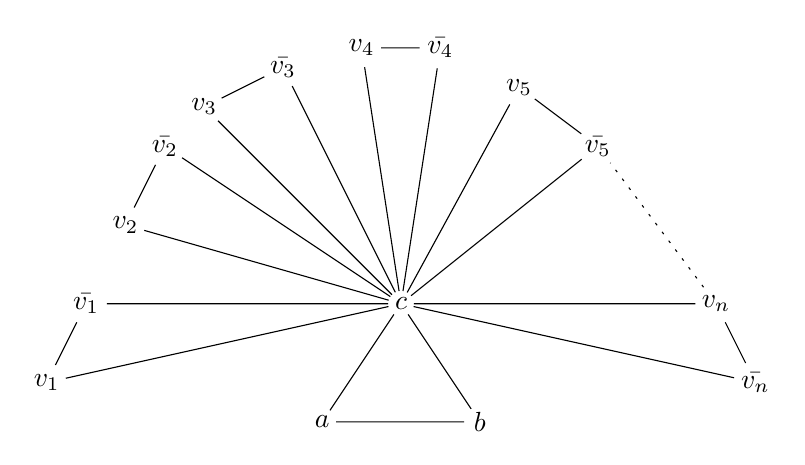
\begin{tikzpicture}
\node[circle,inner sep=1pt,minimum size=1mm] (v1) at (-4,-2.5) {$v_1$};
\node[circle,inner sep=1pt,minimum size=1mm] (nv1) at (-3.5, -1.5) {$\bar{v_1}$};
\node[circle,inner sep=1pt,minimum size=1mm] (v2) at (-3,-0.5) {$v_2$};
\node[circle,inner sep=1pt,minimum size=1mm] (nv2) at (-2.5, 0.5) {$\bar{v_2}$};
\node[circle,inner sep=1pt,minimum size=1mm] (v3) at (-2,1) {$v_3$};
\node[circle,inner sep=1pt,minimum size=1mm] (nv3) at (-1, 1.5) {$\bar{v_3}$};
\node[circle,inner sep=1pt,minimum size=1mm] (v4) at (0,1.75) {$v_4$};
\node[circle,inner sep=1pt,minimum size=1mm] (nv4) at (1, 1.75) {$\bar{v_4}$};
\node[circle,inner sep=1pt,minimum size=1mm] (v5) at (2,1.25) {$v_5$};
\node[circle,inner sep=1pt,minimum size=1mm] (nv5) at (3, 0.5) {$\bar{v_5}$};
\node[circle,inner sep=1pt,minimum size=1mm] (vn) at (4.5,-1.5) {$v_n$};
\node[circle,inner sep=1pt,minimum size=1mm] (nvn) at (5, -2.5) {$\bar{v_n}$};
\node[circle,inner sep=1pt,minimum size=1mm] (c) at (0.5, -1.5) {$c$};
\node[circle,inner sep=1pt,minimum size=1mm] (a) at (-0.5, -3) {$a$};
\node[circle,inner sep=1pt,minimum size=1mm] (b) at (1.5, -3) {$b$};

\draw (c)--(v1)--(nv1)--(c);
\draw (c)--(v2)--(nv2)--(c);
\draw (c)--(v3)--(nv3)--(c);
\draw (c)--(v4)--(nv4)--(c);
\draw (c)--(v5)--(nv5)--(c);
\draw (c)--(vn)--(nvn)--(c);
\draw (c)--(a)--(b)--(c);

\draw [dash pattern={on 1pt off 3pt}](vn) --(nv5);
\end{tikzpicture}
\end{center}
\vspace{1cm}
\end{frame}
\begin{frame}
If the graph $G_\varphi$ is $3$-colored, vertices $a$ and $b$ should have different colors, we will call the assigned colors to these two vertex $T$ (True) and $F$ (False) respectively. Then each pair $v_i$ and $\bar{v_i}$ should have colors $T$ and $F$ (or $F$ and $T$) respectively. We can interpret this as a truth assignment to the literals. We call the assigned color to the vertex $c$, color $N$ (Neutral). For easiness, will call the vertices $a$, $b$ and $c$ by their colors $T$, $F$ and $N$ respectively. We should expand the graph to include the clauses. We construct a small OR-gadget graph for each clause $Cj = (x \lor y\lor z)$ in $\varphi$:

\begin{center}
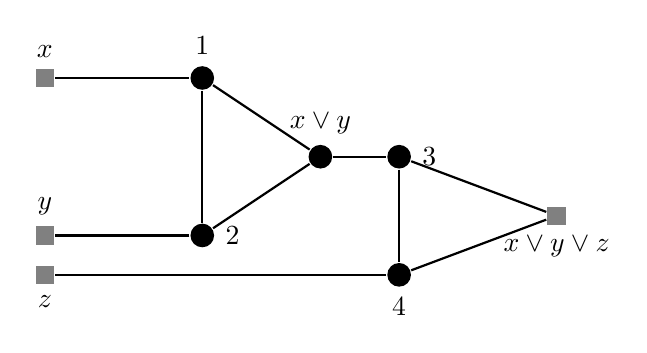
\begin{tikzpicture}[
       thick,
       acteur/.style={
         circle,
         fill=black,
         thick,
         inner sep=2pt,
         minimum size=0.2cm
       }
     ] 
\node[label=$x$,fill=gray] (x) at (-4.5,2.5) {};
\node[label=$y$,fill=gray] (y) at (-4.5, 0.5) {};
\node[label=below:$z$,fill=gray] (z) at (-4.5,0) {};
\node[label=above:1,circle,fill=black,inner sep=1pt,minimum size=3mm] (1) at (-2.5, 2.5) {};
\node[label=right:2,circle,fill=black,inner sep=1pt,minimum size=3mm] (2) at (-2.5,0.5) {};
\node[label=$x\lor y$,circle,fill=black,inner sep=1pt,minimum size=3mm] (xy) at (-1, 1.5) {};
\node[label=right:3,circle,fill=black,inner sep=1pt,minimum size=3mm] (3) at (0,1.5) {};
\node[label=below:4,circle,fill=black,inner sep=1pt,minimum size=3mm] (4) at (0, 0) {};
\node[label=below:$x\lor y\lor z$,fill=gray] (xyz) at (2,0.75) {};

\draw (x)--(1)--(2)--(y);
\draw (1)--(xy)--(2);
\draw (xy)--(3)--(4)--(z);
\draw (3)--(xyz)--(4);

\end{tikzpicture}
\end{center}
\vspace{1cm}


For inputs $x$, $y$ and $z$, the gadget results $(x \lor y\lor z)$:

In a $3$-coloring, 

\begin{itemize}

\item if we color $x$, $y$, $z$ with color $F$ (false), then one of vertices $1$ and $2$ should be colored with $T$ and the other one with $N$, hence $x\lor y$ should be colored with $F$, therefore one of the vertices $3$ and $4$ should have the color $T$ and the other one color $N$. It results the color $F$ for the output $x\lor y\lor z$ as it was desired.


\item if we color at least one of the input vertices with the color $T$, the output $x\lor y\lor z$ gets the color $T$. We don't check it here.
\end{itemize}

Now, for each clause $C_j$, we connect its correspondence OR-Gadget to vertex $F$ and $N$ from the triangle.

\begin{center}
%\tikzset{test/.style={circle, draw=black}}
%\begin{figure}

\begin{tikzpicture}

%\begin{element}[place at cordinate (0,4), scale=1]
%\begin{tikzpicture}[scale=1, every node/.style={scale=1}]
\node[circle,inner sep=1pt,minimum size=1mm] (v1) at (-4,-2.5) {$v_1$};
\node[circle,inner sep=1pt,minimum size=1mm] (nv1) at (-3.5, -1.5) {$\bar{v_1}$};
\node[circle,inner sep=1pt,minimum size=1mm] (v2) at (-3,-0.5) {$v_2$};
\node[circle,inner sep=1pt,minimum size=1mm] (nv2) at (-2.5, 0.5) {$\bar{v_2}$};
\node[circle,inner sep=1pt,minimum size=1mm] (v3) at (-2,1) {$v_3$};
\node[circle,inner sep=1pt,minimum size=1mm] (nv3) at (-1, 1.5) {$\bar{v_3}$};
\node[circle,inner sep=1pt,minimum size=1mm] (v4) at (0,1.75) {$v_4$};
\node[circle,inner sep=1pt,minimum size=1mm] (nv4) at (1, 1.75) {$\bar{v_4}$};
\node[circle,inner sep=1pt,minimum size=1mm] (v5) at (2,1.25) {$v_5$};
\node[circle,inner sep=1pt,minimum size=1mm] (nv5) at (3, 0.5) {$\bar{v_5}$};
\node[circle,inner sep=1pt,minimum size=1mm] (vn) at (4.5,-1.5) {$v_n$};
\node[circle,inner sep=1pt,minimum size=1mm] (nvn) at (5, -2.5) {$\bar{v_n}$};
\node[circle,inner sep=1pt,minimum size=1mm] (n) at (0.5, -1.5) {$N$};
\node[circle,inner sep=1pt,minimum size=1mm] (t) at (-0.5, -3) {$T$};
\node[circle,inner sep=1pt,minimum size=1mm] (f) at (1.5, -3) {$F$};

\draw (n)--(v1)--(nv1)--(n);
\draw (n)--(v2)--(nv2)--(n);
\draw (n)--(v3)--(nv3)--(n);
\draw (n)--(v4)--(nv4)--(n);
\draw (n)--(v5)--(nv5)--(n);
\draw (n)--(vn)--(nvn)--(n);
\draw (n)--(t)--(f)--(n);


\draw [dash pattern={on 1pt off 3pt}](vn) --(nv5);

\begin{scope}[shift={(1.5,-5.5)},rotate=90,scale=0.5, every node/.style={scale=0.5}]

{[
       thick,
       acteur/.style={
         circle,
         fill=black,
         thick,
         inner sep=2pt,
         minimum size=0.2cm
       }

\node[label=$x_3$,fill=gray] (x) at (-4.5,-7.5) {};
\node[label=$y_3$,fill=gray] (y) at (-4.5, -9.5) {};
\node[label=below:$z_3$,fill=gray] (z) at (-4.5,-10) {};
\node[label=above:1,circle,fill=black,inner sep=1pt,minimum size=3mm] (1) at (-2.5, -7.5) {};
\node[label=right:2,circle,fill=black,inner sep=1pt,minimum size=3mm] (2) at (-2.5,-9.5) {};
\node[label=$x_3\lor y_3$,circle,fill=black,inner sep=1pt,minimum size=3mm] (xy) at (-1, -8.5) {};
\node[label=right:3,circle,fill=black,inner sep=1pt,minimum size=3mm] (3) at (0,-8.5) {};
\node[label=below:4,circle,fill=black,inner sep=1pt,minimum size=3mm] (4) at (0, -10) {};
\node[label=below:$x_3\lor y_3\lor z_3$,fill=gray] (xyz1) at (2,-8.75) {};

\draw (x)--(1)--(2)--(y);
\draw (1)--(xy)--(2);
\draw (xy)--(3)--(4)--(z);
\draw (3)--(xyz1)--(4);
\draw [red] (f)--(xyz1)--(n);
   
   
{[
       thick,
       acteur/.style={
         circle,
         fill=black,
         thick,
         inner sep=2pt,
         minimum size=0.2cm
       }
     ] 
\node[label=$x_2$,fill=gray] (x) at (-4.5,2.5) {};
\node[label=$y_2$,fill=gray] (y) at (-4.5, 0.5) {};
\node[label=below:$z_2$,fill=gray] (z) at (-4.5,0) {};
\node[label=above:1,circle,fill=black,inner sep=1pt,minimum size=3mm] (1) at (-2.5, 2.5) {};
\node[label=right:2,circle,fill=black,inner sep=1pt,minimum size=3mm] (2) at (-2.5,0.5) {};
\node[label=$x_2\lor y_2$,circle,fill=black,inner sep=1pt,minimum size=3mm] (xy) at (-1, 1.5) {};
\node[label=right:3,circle,fill=black,inner sep=1pt,minimum size=3mm] (3) at (0,1.5) {};
\node[label=below:4,circle,fill=black,inner sep=1pt,minimum size=3mm] (4) at (0, 0) {};
\node[label=below:$x_2\lor y_2\lor z_2$,fill=gray] (xyz2) at (2,0.75) {};

\draw (x)--(1)--(2)--(y);
\draw (1)--(xy)--(2);
\draw (xy)--(3)--(4)--(z);
\draw (3)--(xyz2)--(4);  
\draw [red](f)--(xyz2)--(n);

{[
       thick,
       acteur/.style={
         circle,
         fill=black,
         thick,
         inner sep=2pt,
         minimum size=0.2cm
       }
     ] 
\node[label=$x_1$,fill=gray] (x) at (-4.5,12.5) {};
\node[label=$y_1$,fill=gray] (y) at (-4.5, 10.5) {};
\node[label=below:$z_1$,fill=gray] (z) at (-4.5,10) {};
\node[label=above:1,circle,fill=black,inner sep=1pt,minimum size=3mm] (1) at (-2.5, 12.5) {};
\node[label=right:2,circle,fill=black,inner sep=1pt,minimum size=3mm] (2) at (-2.5,10.5) {};
\node[label=$x_1\lor y_1$,circle,fill=black,inner sep=1pt,minimum size=3mm] (xy) at (-1, 11.5) {};
\node[label=right:3,circle,fill=black,inner sep=1pt,minimum size=3mm] (3) at (0,11.5) {};
\node[label=below:4,circle,fill=black,inner sep=1pt,minimum size=3mm] (4) at (0,10) {};
\node[label=below:$x_1\lor y_1\lor z_1$,fill=gray] (xyz3) at (2,10.75) {};

\draw (x)--(1)--(2)--(y);
\draw (1)--(xy)--(2);
\draw (xy)--(3)--(4)--(z);
\draw (3)--(xyz3)--(4); 
\draw [red](f)--(xyz3)--(n); 
\end{scope}
\draw [dash pattern={on 1pt off 4pt}] (7,-6.5)--(9,-6.5)
\end{tikzpicture}
%\end{element}
%\end{tikzpicture}
 
%\end{figure}
\end{center}
\vspace{1cm}

and at last, we connect every literal from each clause in OR-gadget to its correspondence vertex $v_i$ or for negation of a literal to its correspondence vertex $\bar{v_i}$

Now, the graph $G_\varphi$ is ready. We will prove that it is $3$-colorable iff $\varphi$ is satisfiable:

\begin{itemize}
\item $\varphi$ is satisfiable implies $G_\varphi$ is $3$-colorable:

\begin{itemize}
\item $\varphi$ is satisfiable, means that its all clauses are "True" and therefore every OR-gadget in $G_\varphi$ resluts $T$ color. 

\item If literal $t_i$ has truth value "True", we color $v_i$ with $T$ and $\bar{v_i}$ with $F$. 

Concerning the figure, the graph is $3$-colorable. 

\end{itemize}
\item $G_\varphi$ is $3$-colorable implies $\varphi$ is satisfiable.
\begin{itemize}
\item If $v_i$ is colored $T$ and hence $\bar{v_i}$ is colored $F$, we set $t_i$ to "True" and therefore negation of it to "False", that is a valid assignment.

\item Because of $3$-colorability of the graph, output of every OR-gadget should be colored $T$ because it is connected to vertices with colors $F$ and $N$, Hence at least one of input vertices of each OR-gadget is colored $T$, then $\varphi$ is satisfiable. 
\end{itemize}
\end{itemize}

\end{proof}


DSATUR is a graph coloring algorithm created by Daniel Br\'elaz \cite{brelaz} in 1979. Algorithm DSATUR is one of several heuristic algorithms which try to find the best possible solution by ordering nodes properly before the greedy search. The Greedy coloring method is the simplest algorithm which takes an ordering of nodes of a graph and colors these with the smallest possible color. 

Turner \cite{turner} proved that the run time for the heuristic algorithm DSATUR could be $\mathcal{O}(m \log n)$, for a graph with $n$ vertices and $m$ edges.

At first, one definition is needed:

\begin{defi}
Let $G$ be a simple and partially colored graph. The saturation degree of a vertex is the number of different colors to which it is adjacent (colored vertices).\cite{brelaz}
\end{defi}

In DSATUR algorithm (from {\bf d}egree {\bf sat}uration), nodes with higher degree of saturation are picked first, this yields a specific ordering of nodes for backtracking.

\vspace{1cm}

\begin{algorithm}[H]
\SetAlgoLined
\DontPrintSemicolon
  \caption{DSATUR (so called because it uses saturation degree)\cite{brelaz}}

  Arrange the vertices by decreasing order of degrees.\;
   Color a vertex of maximal degree with color $1$.\;
  Choose a vertex with a maximal saturation degree. If there is an
equality, break the tie by choosing any vertex of maximal degree in the uncolored
subgraph.\;
    Color the chosen vertex with the least possible (lowest numbered)
color.\;
  If all the vertices are colored, stop. Otherwise, return to step 3.\;
 
\end{algorithm}

\newpage

DSATUR algorithm in its original form is not an exact algorithm and not much useful for our purpose in this paper. 

There are several inhancements and variation, all based on DSATUR. One of them is "DSATUR-based Branch-$\&$-Bound" which gives an exact solution, optimized by node ordering proposed by DSATUR. This algorithm is used in this thesis.

If the vertices are being colored successively with the least possible color in a
given order, the coloration is started from a clique. (lower bounds on the 
chromatic number.)

In exact algorithm, in first step we begin to color with the biggest clique in the DSATUR algorithm.



\newpage
\newgeometry{left=1in,right=1.2in,top=1in,bottom=1in}
\begin{algorithm}[H]
\SetAlgoLined
\DontPrintSemicolon
  \caption{Randall-Brown's Modified Algorithm\cite{randall}}
  
{\small  Find a maximal clique $K$. Let dimension of clique is $w$. By using DSATUR
beginning with this clique, find an initial coloration with $r$ colors (an
upper bound) and a rank (coloration) order of the vertices. If $w = r$ , stop.\\

 Color the vertices of the clique $K$ with $1, 2, . . . w$ successively. For each
vertex $v$ in $G$ let $U(v) \in \{1, 2, . . . r + 1\}$ is the set of colors which can color
$v$. For each vertex $x_k$ out of the clique, let $U(x_k) = U(x_k) - j$ where $j$ is
the color of a vertex in $K$ which is adjacent to $x_k$.\\

 Let $k = w + 1$ and $q = r$.\newline
$U(x_k)$ is upper-limited by color $q - 1$ and each vertex is limited by the color
with the same cardinality as its rank). Color $x_k$ with the least possible
color and remove this color from $U(x_k)$ and the color list of all vertices
which are adjacent to $x_k$ , until there is a modification of the $x_k$ color.

 Let $k = k + 1$ and determine $U(x_k)$.\\

 If $U(x_k) = \infty$ go to step 10. Otherwise let $i$ be the least color of $U(x_k)$ and
color $x_k$ with $i$ and $U(x_k) = U(x_k) - i$ then remove this color from the
color set of all vertices adjacent to $x_k$ (with greater rank) until there is a
modification of $x_k$ color. If $i \geq q$ go to step 8.\\

 If $k = n$ , let $q = L$ where $L$ is the number of colors used for this coloration
and go to step 7, otherwise go to step 4.\\

 If $q = w$, stop. Otherwise , let $x_j$ be the $q$-colored vertex with minimal
rank. If the rank of $x_j$ is equal to $w + 1$ , stop, otherwise let $k = j - 1$ and
go to step 5.\\

 If $k = w + 1$ stop. Otherwise, label all unlabeled vertices which have the
following properties:
\begin{enumerate}[(i)]
\item with rank $< k$,

\item adjacent to $k$,

\item with none of the colors of vertices of the clique adjacent to $k$ , and
\item with minimal rank among all vertices of their color which are adjacent
to $k$.
\end{enumerate}\newline
Now let $\nu = k$ . For those vertices are labeled with $k$, if we obtain the rank
$k$ or more in a partial coloration, the label should be removed.\\


\nl Let $k = t$ where $t$ is the maximal rank of labeled vertices, which have rank $< k$. For $k < i \leq \nu$ , $U(x_i)$ is the set of colors defind in step 3. Go to step 5.\\


\nl If none of the colors is possible for $x_k$ (all are tested), then backtracking
should be done. For this go to step 8.\\}
\end{algorithm}
\restoregeometry

\end{document}
}